% !TEX encoding = Windows Latin 1
\documentclass{llncs}
\usepackage{graphicx}
\usepackage[english]{babel}
\usepackage{color}
\usepackage{ucs}
\usepackage[latin1]{inputenc}
\usepackage{amsmath}
\usepackage{mathtools} 

\newcommand{\markus}[1]{\textcolor{red}{Markus: #1}}
\newcommand{\arif}[1]{\textcolor{blue}{Arif: #1}}
\newcommand{\lars}[1]{\textcolor{greed}{Lars: #1}}
\newcommand{\tinyparagraph}[1]{\vspace{0.2cm}\noindent\textbf{#1: }}

\renewcommand\floatpagefraction{.9}
\renewcommand\topfraction{.9}
\renewcommand\bottomfraction{.9}
\renewcommand\textfraction{.1}   
\setcounter{totalnumber}{50}
\setcounter{topnumber}{50}
\setcounter{bottomnumber}{50}

\bibliographystyle{splncs03}

\begin{document}
\frontmatter        
\pagestyle{headings}
\mainmatter           

%\title{Automated and Transparent Model Fragmentation for Persisting Large Models}
\title{Automated and Transparent Model Fragmentation for Persisting Large Models}

\author{Markus Scheidgen and Anatolij Zubow}
\authorrunning{M. Scheidgen, A. Zubow}
\institute{Department of Computer Science, Humboldt Universit�t zu Berlin\\
           Unter den Linden 6, 10099 Berlin, Germany\\
           \email{\{scheidge,zubow\}@informatik.hu-berlin.de}}

\maketitle
%\thispagestyle{empty}

\begin{abstract} 
Existing model persistence frameworks either store models as a whole or object by object. Since most modeling tasks work with larger aggregates of a model, existing persistence frameworks either load too many objects or access many objects individually. We propose to persist a model broken into larger fragments.

First, we assess the size of large models and describe typical usage patterns to show that most applications work with aggregates of model objects. Secondly, we provide an analytical framework to assess execution time gains for partially loading models fragmented with different granularity. Thirdly, we propose meta-model-based fragmentation that we implemented in an EMF based framework. Fourthly, we analyze our approach in comparison to other persistence frameworks (XMI, CDO, and Morsa) based on four common modeling tasks: create/modify, traverse, query, and partial loads.

We show that there is no generally optimal fragmentation, that fragmentation can be achieved automatically and transparently, and that fragmentation provides considerable performance gains compared to other persistence strategies.
\end{abstract}

\section{Introduction}

\subsection{Problem Statement}
Large models (directed labelled graphs with a inherent spanning tree) cannot be maintained in computer memory. Large models need to be fragmented into smaller models. These smaller parts can be loaded and worked with. This is practical, since most applications only require to handle a small part of a large model at a time. 

We distinguish between large and \emph{extra large} models. Large models are to big for computer memory, but still small enough to be served from a single computer: large models are small enough for common hard drives and a single computer can bear the load from accessing the model (small number of users, infrequent access, only small chunks are accessed). Extra large models require a distributed data store, because they are either to big or are used in a way that a single computer can not handle the load. Safety, redundancy, dependability, etc. are other qualities that we associate with extra large models and their storage. 

Modern key value data stores, can (in principle) store extra large models. They provide all necessary qualities associated with extra large models (distributed, safe, redundant, dependable, scalability, etc.). The problem is that models have to be fragmented so that they can be accessed in part. The concrete fragmentation of a model and its granularity directly influences the performance of storing, accessing, and working with the model. Here, performance regards execution time, CPU load, and RAM memory usage. 

\subsection{Fragmentation}

Models (or data, or information) in this paper are directed labelled graphs (with an inherent spanning tree). Common model representations are EMF-based models or XML documents. We assume that nodes and all their outgoing edges always belong together and are inseparable\footnote{This is in direct contrast to ER/SQL based models and stores, where links between entities are stored in separate tables}. Often we will only write about nodes, but also mean all their outgoing edges (references to other nodes). For that matter a model is just a set of nodes (objects).

A \emph{fragmentation} of a model is a set of sets of objects. The union of all sets in a fragmentation is the model; all sets are disjunct. The sets in a fragmentation are called \emph{fragments}. The objects in each fragment contain a single spanning tree (sub tree of the models spanning tree). Each fragment is identified by a unique key. The fragment key identifies the root of that tree. Model edges can be associated with keys to reference objects in a different fragment.  

\subsection{Existing Storage Solutions and Fragmentation Strategies}

There are three existing fragmentation strategies:
\begin{itemize}

\item \emph{No fragmentation}, the model is not fragmented. Large models are not possible.
\item \emph{Total fragmentation}, each object of the model (a node with all its outgoing edges) is stored in its own fragment.
\item \emph{Manual fragmentation}, the user determines which objects of a model comprise which fragments.
\end{itemize} 

\subsection{Key Value Stores}

Key value stores technical systems that persist large (hash-)maps. They can store arbitrary values (string or byte arrays) under arbitrary keys (string or byte arrays). There are different mature solutions for different environments (grid, cluster, cloud). A key-value combination is called \emph{entry}.

Key value stores can be \emph{distributed} or \emph{non distributed}; they can be \emph{ordered} or {unordered}. Generally values access complexity is logarithmic to the size the stored map (number of keys). This is true for both non distributed and distributed stores. In distributed stores complexity also depends logarithmically on the size of the store (number of computers (nodes) in the store). Reading an access value is linear to the size of the value. In distributed stores is a possibility to read values in parallel. In ordered stores, subsequent keys of an already accessed key can be accessed in constant time (scan). In general models are serialized and need parsing to be used. A loaded value (model fragment) is parsed in linear time (depending on the fragments size). We assume that parsing can only be performed on the client and no parallel parsing on different computers is possible. 

\subsection{Detailed Problems}

There are several distinct problems with fragmentation of (extra) large models:
\begin{itemize}
\item Trivial fragmentation (no or total) might not produce optimal or even functional results. 

\item In extreme broad models one object might be too big (too many outgoing edges). Too big to be stored in RAM memory, or too big for reasonable and efficient use. This happens for example with sensor data collected over long periods of time. On sensor (object, node) holds references (edges) to thousands of thousands of values.  

\item There are several parameters that influence optimal fragmentation: parsing speed, data store access speed, whether parsing or accesses different entries can be parallelized (distribute scenario). Random access (random read) vs. sequential access (scan). 

\item Fragmentation in general depends on model usage patterns. These cannot be known at model creation and might change over time.
\end{itemize}

\subsection{Terms}

Specific terms are: \emph{model}, \emph{large model}, \emph{extra large model}, \emph{fragmentation}, \emph{fragment}, \emph{no fragmentation}, \emph{total fragmentation}, \emph{manual fragmentation}, \emph{key-value data store}, \emph{entry}, \emph{key}, \emph{value}, \emph{(un-)ordered store}, \emph{(non-)distributed store}. Further terminology may be introduced later.


\section{Applications for Large Models}
\label{sec:applications}

In this section, we look at examples for three modeling applications. We do this for two reasons. The first reason is to discuss the actual practical relevance of large models. The second reason is to identify model usage patterns: which of the four modeling tasks (create, traverse, query, partial load) are actually used, in what frequency, and with what parameters. At the end of this section, we provide a tabular summary of our assessment.

%The first one is software modeling, which is what most of the MODELS community is concerned with and what the modeling frameworks mentioned in this paper were designed for. But techniques originally developed for software modeling are also used for other applications. More abstractly, software modeling can be explained as the representation, analysis, and manipulation of structured data. 
%
%Our research group, for example, uses EMF to represent and analyse sensor data received from our wireless sensor network test-bed (\emph{Humboldt Wireless Lab}~\cite{hwl}). Models of heterogeneous sensor data will be our second application. 
%This application is what actually motivated us as authors for this work, because existing approaches where either impractical (lazy loading of EMF resources), or far to slow to store the data at the rate it was produced (CDO and manual relational data base persistence). 
%Refer to~\cite{clickwatch} for more details. 
%
%The third application that we want to analyse, are geo-spatial models and more specifically 3D object models of cities. Such models represent the features of a city (boroughs, streets, buildings, floors, rooms, windows, etc.) as a containment hierarchy of objects and their properties. 
%These models are closely related to sensor data analysis.
%
%For all three applications, we estimate the size of typical models. Furthermore, we determine the most important use cases for all three applications. From these use cases we derive the commonly used modeling tasks and their characteristics.

\subsection{Software Models}
Model Driven Software Development (MDSD) is the application that modelling frameworks like EMF were actually designed for. In MDSD all artifacts including traditional software models as well as software code are understood as models~\cite{modelsAsCode}, i.e. directed labelled graphs of typed nodes with an inherent containment hierarchy. 
%IDEs (e.g. eclipse's JDT or CDT) already represent code as models (ASTs). Advances in modeling frameworks (e.g. model comparison) suggests that code is also persisted as model.

\subsubsection*{Model Size}

Since models of software code (code models) provide the lowest level of abstraction, we assume that models of software code are the largest software models. Therefore, software projects with a large code base probably provide the largest examples for software models. We will first look at the Linux Kernel as an example for a large software project and then extend our estimates on other operating system projects.

Traditionally code size is measured in \emph{lines of code} LOC (physical lines), SLOC (source LOC, like LOC but without empty lines, comments, duplicates), and LLOC (logical LOC, like SLOC but normalized to one statement per line).~\cite{wheeler} 
These measures exist for many known software projects (and their history) and can be easily captured for open source projects. 

To estimate the size of code models in number of objects, we additionally need to know how many model objects constitute an average LOC. We used the C Development Toolkit (CDT) to parse the current version of the Linux Kernel (3.2.1) and count the number of abstract syntax tree (AST) nodes required. We assume that model objects and AST nodes are equivalent for our estimation. We also counted the LOCs of the Kernel's code with \emph{sloccount}. This provides an model objects per LOC ratio of 5.99 that we use for all further estimates.

From the GIT versioning system we learned the average numbers of added, removed, and manipulated LOCs per month based on last year's history (4,300 LOC added, 1,800 LOC removed, and 1,500 LOC modified per day). We extrapolate these numbers to estimate the older history of the Kernel. Based on the actual grow in LOC over the last years and our model objects per LOC ratio, we calculated the average number of modified objects in a modified LOC, and can finally estimates the number of all objects in the Kernel's code including its history. This is a model that only contains the changes.

\begin{figure}
  \centering
  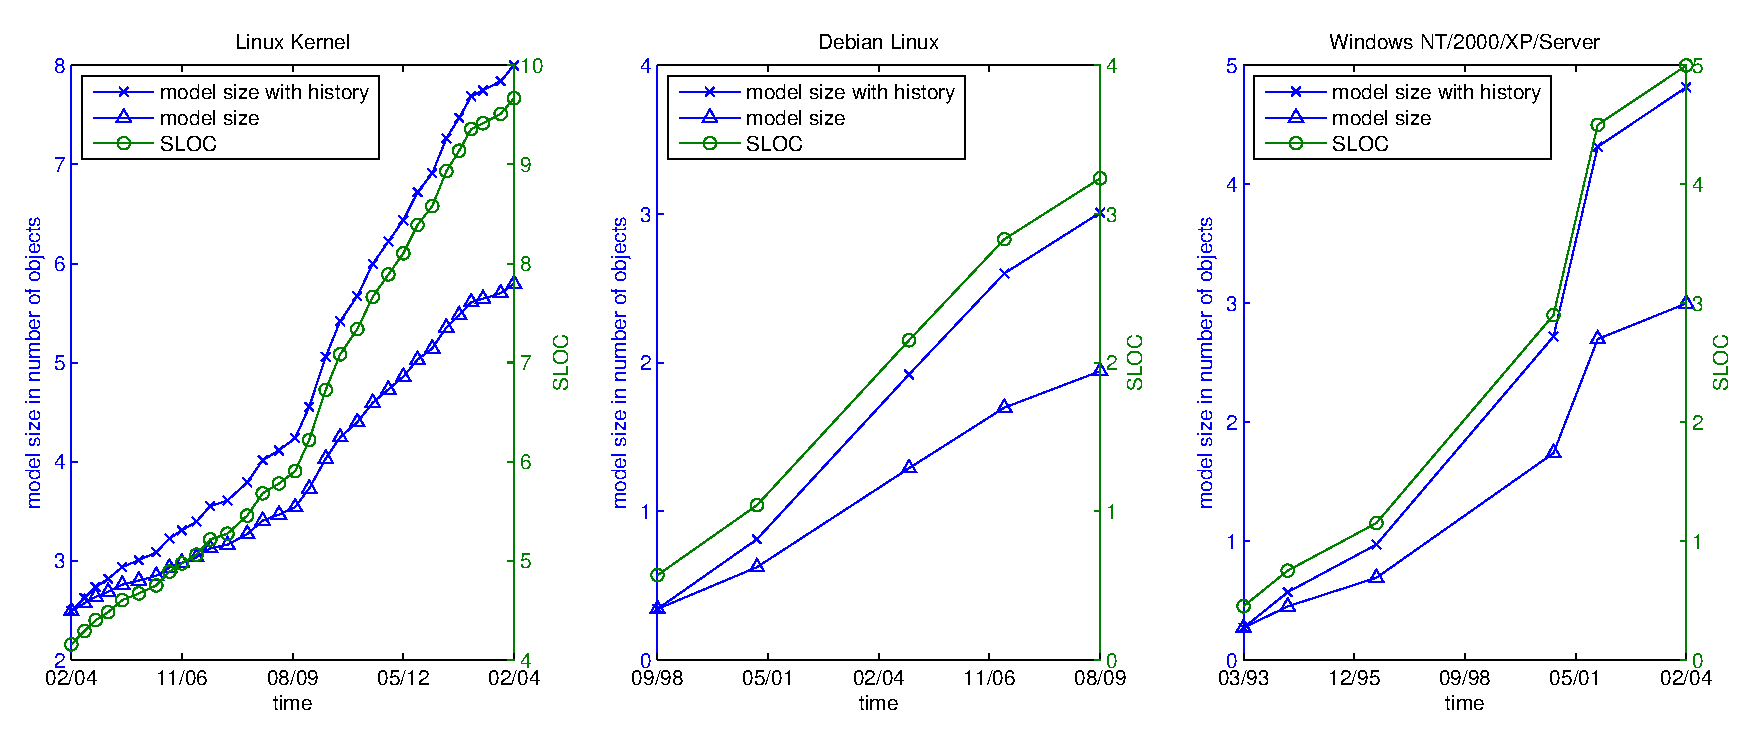
\includegraphics[width=\linewidth]{figures/software_model_sizes}
  \caption{Rough estimates for software code model sizes based on actual SLOC counts for existing software projects.}
  \label{fig:software_model_sizes}
\end{figure}


We also transferred all ratios from the Kernel to other OS software projects and publicly reported LOC counts. The results represent rough estimates and are presented in Fig.~\ref{fig:software_model_sizes}. As you can see, these large software models can have a size upto a magnitude of $10^9$ objects.

Furthermore, it is not clear whether further growth in software project size is exponential or linear. Some believe that software size follows Moore's Law. Others think that software is bound by increasing complexity and not by the limitations of underlying hardware.

\subsubsection*{Usage Patterns}
There are two major use cases in today's software development: editing and transforming or compiling. The first use case is either performed on diagrams (graphical editing) or on compilation units (e.g. Java-files, textual editing). Diagram contents roughly corresponds to package contents. Both packages and compilation units are sub-trees within the containment tree of a software model.  Transformations or compilations are usually either done for the whole model or again on a per package or compilation unit basis. Within these aggregates, the (partial) model is traversed. A further use-case is analysis. Analysis is sometimes performed with single queries. But due to performance issues, model analysis is more often performed by traversing the model and by executing multiple queries with techniques similar to model transformations. Software models are only accessed by a view individuals at the same time.

%\subsubsection{What are software code models?}
%We use the term model to describe MDSD artifacts. Originally these artifacts were models on a high level of abstraction, but today programming code, can also be understood as models. For example IDEs such as eclipse JDT or eclipse CDT internally maintain programming code as ASTs (primitive models) in order to provide advanced IDE features such as outlines, error annotations, type and call hierarchies, and code completion. It is safe to assume that programming code contains far more information compared to high-level models. Since we are looking for extra large models, we will concentrate on software code models.
%
%Advances in language workbenches suggest to replace these IDEs with eclipse EMF based and generated tools. Advances in comparison and versioning of models will soon allow to replace per-line-text-file-based versioning systems (e.g. CSV, SVN, GIT) with model based (e.g. EMF-based) systems that version on a per mode-object- or even per-object-attribute basis.
%
%\subsubsection{How big is are existing software code models?}
%How large are these software code models? Traditionally code size is measured in \emph{lines of code} LOC (physical lines), SLOC (source LOC, like LOC but without empty lines, comments, duplicates; refer to Wheeler~\cite{wheeler}, and LLOC (logical LOC, like SLOC but normalized to one statement per line). These measures exist for many known software projects (and their history) and can be easily captured for open source projects. 
%
%In order to determine corresponding model sizes, we need to know how much model objects each LOC represents. To estimate this, we used the eclipse CDT parser as tool and the linux kernel as sample. The CDT parser is specialized to parse C/C++ code in its un-preprocessed form. Thus, the resulting ASTs are not bloated with information injected (with lots of duplicates) during pre-processing. Of course ASTs are not software models as they are understood in the OMG/EMF world, but we can assume that proper C/C++ models will contain one object for each AST node. \markus{This needs a reference}. Parsing the current kernel version, counting its AST nodes, and comparing this number to the kernel's SLOC number gives us a good estimate for objects per SLOC (at least for the kernel code, probably for all C code, and maybe it is also a good estimate for other similar programming languages, e.g. C\#, Java). We will use this estimate to extrapolate the model size of other kernel versions and other software projects. 
%
%Eventually, we want to store software models and its versions. Of course, we only want to store the differences between versions. A software projects model size is determined by the size of the differences that produced the current software model. To determine this size, we need to know how much LOCs were added, removed, and modified in a software project. To estimate this, we use the versioning system GIT as tool and the linux kernel GIT repository as sample. With gitstats we can determine the number of added, removed, and changed lines throughout the repository history. With these numbers, the estimated objects per SLOC and the recorded SLOCs for different kernel versions we can estimate the model size of a kernel software code model repository. We can also assume that other software projects have a similar proportion of added, removed, and modified lines, and transfer these estimates to other software projects. 
%
%\begin{figure}
%  \centering
%  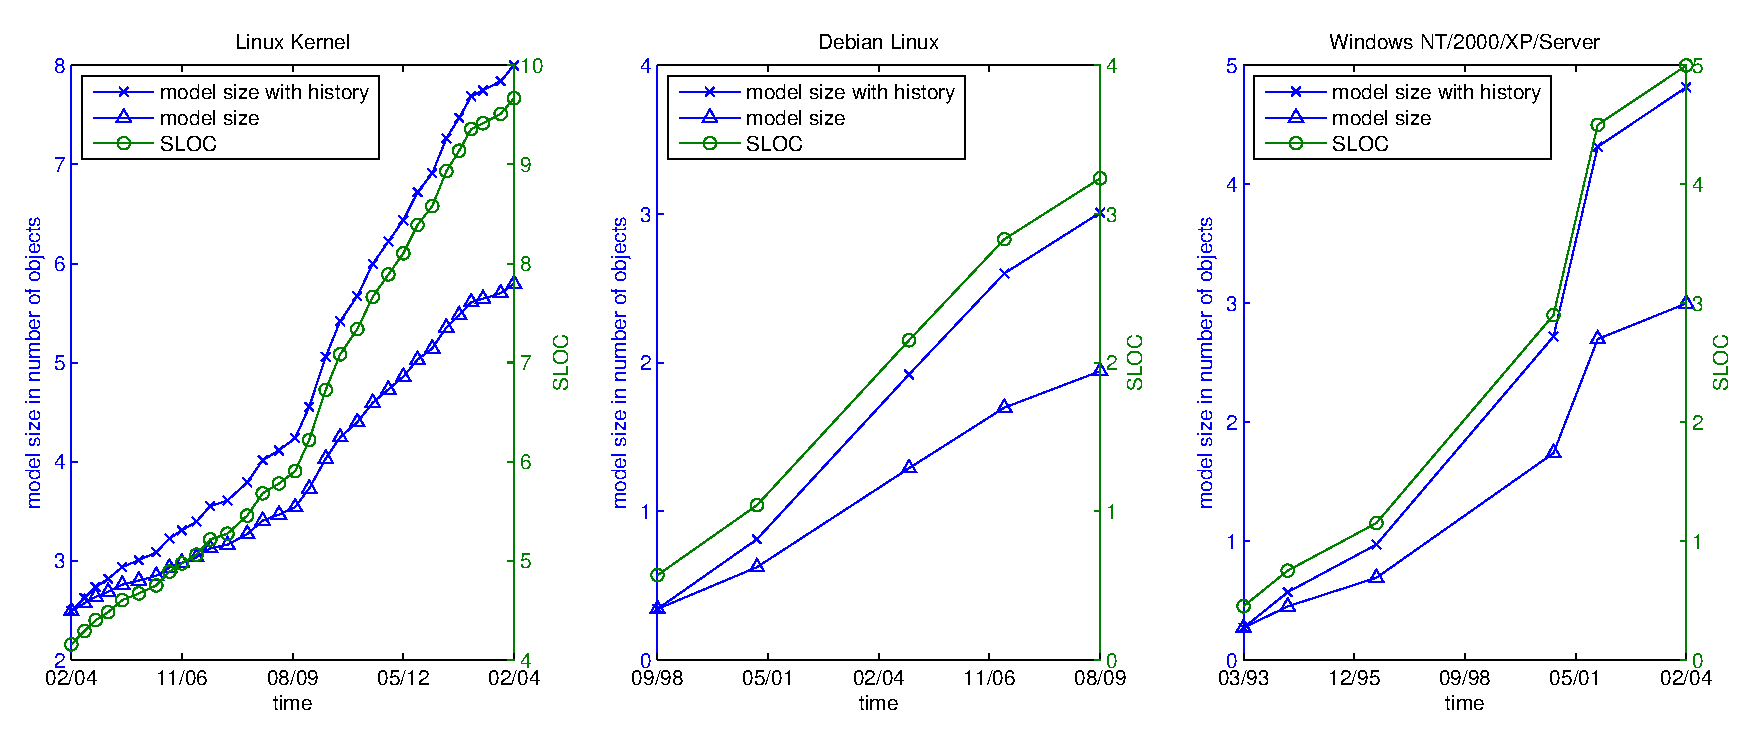
\includegraphics[width=\linewidth]{figures/software_model_sizes}
%  \caption{SLOC and estimated number of objects for popular large software projects.}
%  \label{fig:software_model_sizes}
%\end{figure}
%
%Fig.~\ref{fig:software_model_sizes} shows the LOC numbers and estimated object numbers in corresponding software code models. The charts present different software projects and how size developed over time. \markus{kernel, linux(debian)?, windows - numbers based on kernel git alone, SLOC numbers and transferred kernel estimates.}
%
%\subsubsection{How big are software code models in the future?}
%
%Some believe that the average size software (and software code models for that matter) grows faster than linear following Moore's Law. Maciej Soltysiak for example has analysed the grows of the linux kernel code base and observed exponential growth. A counter argument is that software not only bound by hardware limitations (i.e. Moore's Law) but increasingly by software complexity and therefore will not grow exponentially. Never the less, it is safe to assume that software code models will be larger in the future.

\subsection{Heterogenous Sensor Data}

Sensor data usually comprises of time series of measured physical values in the environment of a sensor; but sensor data can also contain patterns of values (e.g. video images). Sensor data is collected in sensor networks, that combine distributes sensors with an communication infrastructure. Sensor data can be heterogeneous: a sensor network can use different types of sensors that measure a multitude of parameters. \cite{estrin,lynch}. 

Our research group build the \emph{Humboldt Wireless Lab}~\cite{hwl}, a 120 node wireless sensor network. Nodes are equipped with 3 axis accelerometers, but more essentially also produce data from monitoring all running software components (mostly networking protocols), and other system parameters (eg.g. CPU, memory, or radio statistics). We represent and analyse this data as EMF based models (\cite{clickwatch}).
% add cites for SMTL once accepted

\subsubsection*{Model Size}
HWL's network protocols and system software components provide 372 different types of data sets. Each data set is represented as an XML document. Per second each node in the network produces XML entities that translate into an average of 1120 EMF objects. A common experiment with HWL involves 50 nodes and measures of a period of 24h. During such an experiment, the network produces a model of $5*10^9$ objects. 

In general, sensor networks are only bounded by the limitations of the technical infrastructure that supports them. Ambiguous computing and Smart Citys suggest future sensor data models of arbitrary sizes. 

\subsubsection*{Usage Patterns}
There are two major use-cases: recording sensor data and analysing sensor data. Recording sensor data means to store it faster then it is produced. If possible in a manner that supports later analysis. Sensor data is rarely manipulated. Analysis means to access and traverse individual data sets (mostly time series). Each data set or recorded set of data sets is a sub-tree in the sensor data model. Recording and analysis is usually performed by only a single (or a few) individuals at the same time. 

\subsection{Geospatial Models}

3D city models are a good example for structured geo-spatial information. The CityGML~\cite{cityGML} standard, provides a set of xml-schemas (building upon other standards, e.g. GML) that function as a meta-model. CityGML models represent the features of a city (boroughs, streets, buildings, floors, rooms, windows, etc.) as a containment hierarchy of objects. 
%These models are closely related to sensor data analysis.
%CityGML, compared to other quasi standards (e.g. google's KML) does not solely concentrate on 3D measures, but allows to extend the covered information by more semantic attributes (e.g. materials, age, inhabitants, existing infrastructure, etc.).
Geo spatial models usually come in different levels of details (LOD); CityGML distinguishes 5 LODs, 0-4)~\cite{cityGML}. 

\subsubsection{Model Size}
As for many cities, a CityGML model is currently established for berlin~\cite{berlinGML}. The current model of Berlin covers all of Berlin, but mostly on a low-medium level of detail (LOD 1-2). To get an approximation of the model's size, we counted the XML entities. The current Berlin model, contains roughly $128*10^6$ objects. 

Estimated on existing CityGML models published for Berlin~\cite{berlinGML} a LOD 1 building consists of 12.5 objects, a LOD 2 building of 40 objects, and a LOD 3 building of 350 objects. A complete LOD 3-4 model of Berlin would therefore consist of $1*10^9$ objects. Berlin inhabits 3.5 million people. About 50\% of the worlds $7*10^9$ people live in cities. This gives a whole LOD3-4 approximation of $10^{12}$ objects for a \emph{world 3D city model}.

\subsubsection{Usage Patterns}
Compared to model manipulation, model access is far more common and its efficient execution is paramount. If accessed, users usually load a containment hierarchies (sub-tree) corresponding to a given set of coordinates or address (geographic location): partial loads. Queries for distinct feature characteristics within a specific geographic location (i.e. with-in such a partial load) are also common. Geo-spatial models are accessed by many people at the same time. 

\subsection*{Summary}

The following table summarizes this section. Two $+$ signs denote that execution times of the respective tasks are vital for the success of the application; a single $+$ denotes that the task is executed often, but performance is not essential; a $-$ denotes that the task if of minor importance.

\begin{center}
\begin{tabular}{|c||c|c|c|c|c|c|}
\hline
\bf{application} & \bf{model size} & \bf{create/mod.} & \bf{traverse} & \bf{query} & \bf{partial load} \\
\hline\hline
software models & $0-10^9$ & + & ++ & + & + \\
\hline
sensor data & $10^9$ & ++ & ++ & - & ++ \\
\hline
geo-spatial models & $10^9-10^{12}$ & - & - & ++ & ++ \\
\hline
\end{tabular}
\end{center}
\section{Model Fragmentation}
\label{sec:fragmentation}

\subsection{Fragmention in General}
All models considered in this paper can be characterizes as directed labled graphs with a fix spanning-tree called \emph{containment hierarchy}. In EMF based models, the containment hierarchy consists of \emph{containment references}; other graph edges are \emph{cross-references}. 

Model fragmentation approach, breaks (i.e. \emph{fragments}) a model along its containment hierarchy. All \emph{fragments} are disjoint; no object is part of two fragments. Fragmentation is also always complete, i.e. each object is part of one fragment. The set of fragments of a model is called \emph{fragmentation}. References between fragments are called inter-fragment and references within a fragment are called intra-fragment references.

~\footnote{Based on these characteristics, fragments can be compared to EMF's resources (especially with containment proxies); refer to section~\ref{sec:implemention}, where we use resources to realize fragmentation.} 

\begin{figure}[ht]
\centering
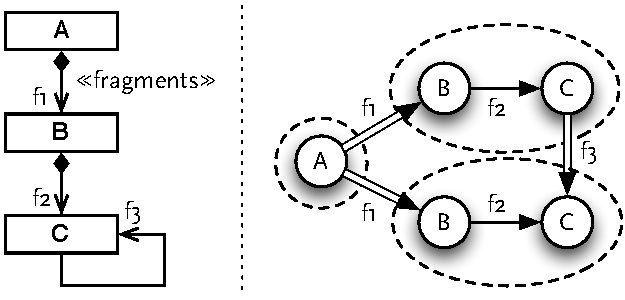
\includegraphics[width=0.65\linewidth]{figures/fragmentationExplained}
\caption{Example meta-model and model. In the mdoel: dashed lines denote fragments, double lines inter- and normal lines intra-fragment references. The references of feature \emph{f1} determine the fragments, the reference of \emph{f3} is a inter-fragment cross-reference by accident.}
\label{fig:metamodelFragmentation}
\end{figure}  

\subsection{Fragmentation Strategies}

Originally a model is not fragmented; once it was fragmented, the fragmentation needs to be maintained when the model is modified. Further, we have to assume that fragmentation has an influence on performance (refer to sections~\ref{sec:gains} and~\ref{sec:evaluation}). We denote a set of algorithms that allows to create and maintain a fragmentation as \emph{fragmentation strategy}.

There are two trivial strategies: \emph{no fragmentation} and \emph{total fragmentation}. No fragmentation means the whole model constitutes of one fragment, such as in EMF (without resources). Total fragmentation means each object constitutes its own fragment. There are as many fragments as objects in the model. This strategy is implemented by existing persistence frameworks like CDO.

\subsection{Meta-Model based Fragmentation}

In this paper, we propose and use \emph{meta-model based fragmentation} as a strategy. A meta-model defines possible models by means of classes ant their attribute and reference features. Whereby, the meta-model determines which reference feature produce containment and with produce cross-references. The meta-modeller already uses containment-reference features to aggregate related objects.

In meta-model based fragmentation, we ask the meta-modeller to additionally mark those containment reference features that should produce inter-fragment containment references. 
This way, the meta-model determines where the containment-hierarchy is broken into fragments, and it becomes easy to create and maintain fragmentations automatically and transparently (ref. to section~\ref{sec:implemention}). Only containment-reference features determine fragmentation, cross-references can become inter-fragment references by accident. See Fig.~\ref{fig:metamodelFragmentation} for an example.

%Only containment features can be designated as inter-fragment reference features and all instances of such a reference feature will be inter-fragment references (like \texttt{a}-references in Fig.~\ref{fig:metamodel_fragmentation_pattern_tree}). Other references (i.e. cross references) can become inter-fragment references \emph{by accident} (like \texttt{c}-references in Fig.~\ref{fig:metamodel_fragmentation_pattern_graph}).


%\subsubsection{Theory}
%Access patterns for a model are strongly influenced by its metamodel.
%Metamodels are tiny in comparison to their large instances. 
%If you imagine looking from above onto a large model, the metamodel types of its objects form patterns. How we access a model is also influenced by its metamodel, since all algorithms doing something with a model are programmed against its metamodel.
%Hence, optimal fragmentation goes along this patterns.
%Most fragments will have the same structure, and fragments are connected through structural features of only few different types.
%One way to define fragmentation is to mark these fragment crossing structural features. 
%
%Fig.~\ref{fig:metamodel_fragmentation_pattern_tree} shows a simple example metamodel type pattern. The instances (links) of feature \emph{a} cross fragment borders (inter fragment links). All other links are intra-fragment links. The situation is a  little more complicated in Fig.~\ref{fig:metamodel_fragmentation_pattern_graph}. Here the links of feature \emph{c} have both inter- and intra-fragment instances. 
%
%If we want to describe fragmentation by marking features as inter- or intra-fragment features, it would work for the example in Fig.~\ref{fig:metamodel_fragmentation_pattern_tree}, but not for the example in Fig.~\ref{fig:metamodel_fragmentation_pattern_graph}. Obviously, we need further restrictions.
%
%Models (as used in this paper) always have a inherent spanning tree. The spanning tree is formed from links that are instances from containment features. All instances of containment features are part of the spanning tree. If we only allow containment features to be inter-fragment features then the instances of inter-fragment feature will always define a unique fragmentation. \markus{Proof?}
%
%\subsubsection{Implementation}
%This describes an implementation based on EMF. 
%
%\subsection{Automated Fragmentation based on Expected Range Queries}
%\subsection{Automated Fragmentation based on Access Patterns}
%\subsection{Fragmentation of Even Models}
%
%\subsubsection{Analysis}
%
%At the beginning, we will look at \emph{even} models. A model is even, if its inner structure suggest fragmentation into equal pieces. For example, an intuitive way to fragment a OO software model is to put each package into one entry. This is an uneven model, since packages have different sizes. Another example is sensor data, sensor data produced at each point in time or on each node has the same size. If one puts each sensor reading or each node into one entry, the entries will have similar size.
%
%Previously, we were looking the gains achieved with optimal fragmentation. While optimal fragmentation is plausible in manually fragmented models for a single specific loaded model (e.g. accessing single sensor readings in ClickWatch). Optimal fragmentation is unlikely for different loaded models (even impossible for models of different size). 
%
%In general, we can assume that the smaller $ope$ is compared to $load$, the more likely it is that much of each entry is part of the loaded model. In other words, the smaller my entries are, the more likely it is that much or all if a single entry is part of the loaded model. We will model $part$  accordingly.
\section{Related Work}
\label{sec:related_work}

\subsection{Model Persistence}
EMF: Models are persisted as XMI documents and can only be used if loaded completely into a computer's main memory. EMF realizes the \emph{no fragmentation} strategy. The memory usage of EMF is linear to the model's size.

There are at least three different approaches to deal with large EMF models: (1) EMF resources, where a resource can be a file or an entry in a database; (2) CDO~\cite{cdo} and other object relational mappings (ORM) for Ecore; (3) morsa~\cite{morsa2011} a EMF data-base mapping for non-relational databases.

First, EMF resources~\cite{emf2009}: EMF allows to fragment a model into different resources. Originally, each resource could only contain a separate containment hierarchy and only inter-resource cross-references were allowed. But since EMF version 2.2 containment proxies are supported. EMF support lazy loading: resources do not have to be loaded manually, EMF loads them transparently once objects of a resource are navigated to. Model objects have to be assigned to resources manually (\emph{manual fragmentation}). To actually save memory the user has to unload resources manually too. The framework MongoEMF~\cite{mongoEMF} maps resources to entries in a MongoDB~\cite{mongodb2010} database.

Secondly, CDO~\cite{cdo}: CDO is a ORM for EMF.~\footnote{Lately, CDO also supports non-relational databases, such as MongoDB~\cite{mongodb2010}. Such features were not evaluated in this paper; but one can assume characteristics similar to those of Morsa.}
It supports several relational databases. Classes and features are mapped to tables and columns. CDO was designed for software modeling and provides transaction, views, and versions.
Relational databases and SQL provide mechanisms to index and access objects with queries. This allows fast queries, if the user understands the underlying ORM.

Thirdly, morsa~\cite{morsa2011}: Different to CDO, Morsa uses mongoDB~\cite{mongodb2010}, a \emph{NoSQL} database that realizes a key-value store (see below). Morsa stores objects, their references and attributes as JSON documents. Morsa furthermore uses mongoDB's index feature to create and maintain indices for specific characteristics (e.g. an objects meta-class reference).

\subsection{Key-Value Stores}

Web and cloud computing require scaleability (replication and sharding\footnote{\emph{Sharding} denotes horizontal partitioning of a database, i.e. to put different parts of the data onto different nodes in the network} in a peer-to-peer network) from a database, and traditional ACID~\cite{ACID} properties can be sacrificed if the data store is easily distributeable. This explains the popularity of \emph{key-value stores}. Such stores provide only a simple map data structure: there are only keys and values. For more information and an comparison of existing key-value stores refer to~\cite{nosql2010}.

Model fragmentation dos not need any complex database structure, since a fragment's content can be serialized (e.g. with XMI) and fragments can be identified by keys (e.g. URIs). Key-value stores on the other hand provide good scaleability for  large models (sharding) or for parallel access (replication).

There are three different applications that inspired three groups of key-value stores. First, there are web applications and the popular MongoDB~\cite{mongodb2010} and CouchDB~\cite{couchdb2010} databases. These use JSON documents as values and provide additional indexing of JSON attributes.

Secondly, there is cloud computing and commercial Google Big-Table~\cite{bigtable2006} and Amazon's Dynamo~\cite{dynamo2007} inspired data stores. HBase~\cite{hbase2008} and Cassandra~\cite{cassandra2009} are respective open source implementations. Those databases strive for massive distribution, they provide no support for indexing inner value attributes, but integrate well into map-reduce~\cite{mapreduce} execution frameworks, such as Hadoop (HBase is Hadoop's native data store). 

A third application is high performance computing. Scalaris~\cite{ScalarisTransactions2008} is a key-value store optimized for massive parallel, cluster, and grid computing. Scalaris provides mechanisms for consistency and transactions and brings some ACID to key-value stores.
\section{Possible Performance Gains from Model Fragmentation}
\label{sec:gains}

In this section, we analyze the theoretically possible execution times of partially loading models with fragmentations of different granularity. This includes an assessments for performance gains from optimal fragmentation strategies compared to no or total fragmentation.

To keep this analysis simple, we have to make two assumptions that will probably seldom hold in reality, but still lead to analysis results that provide reasonable upper bounds for possible gains.
The first assumption: we are only consider fragmentations where all fragments have the same size $f$. 
This means a fragmentation for a model of size $m$ consist of $\lceil m/f \rceil$ fragments\footnote{$\lceil x\rceil$ denotes the ceiling of $x$}. 
The second assumption: all fragmentations are optimal regarding partial loads. This means to load a model part of size $l$, we only need to load $\lceil l/f\rceil$ fragments at most.

To determine the execution time for partial loading depending on the parameters model size $m$, fragment size $f$ and size of the model part $l$, we need two functions that determine the time it takes to read and parse a model and to access a value in a key value store. The read and parse function is linear depending on parsed model size $s$: $parse(s)=\mathcal{O}\left(s\right)$, the access function is logarithmic depending on the number of keys $k$: $access(k)=\mathcal{O}(log(k))$. Most key-value stores, including HBase (that we use for our implementations) provide $\mathcal{O}(log)$ accesses complexity (ref. also to Fig.~\ref{fig:hbaseAccessPerf}).

With the given assumptions, parameters, and functions the time to execute a partial load is:

$$t_{m,f}(l)=\overbrace{\left\lceil\frac{l}{f}\right\rceil}^{\mathclap{\text{number of fragments to load}}}\underbrace{\left(access(\left\lceil\frac{m}{f}\right\rceil) + parse(f)\right)}_{\mathclap{\text{time to load one fragment}}}$$

To actually use this cost function, we need concrete values for $parse$ and $access$. We measured the execution times for $parse$ with EMF's XMI parser for models of various sizes and fit a linear functions to the measured values (Fig.~\ref{fig:emfParsePerf}). For $access$ we measured the execution time for accessing keys in HBase for database tables with various numbers of keys $k$. For $k<10^6$ we use a linear function and for $k\ge 10^6$ a logarithmic function as a fit (Fig.~\ref{fig:hbaseAccessPerf}). 
%For details on the measuring environment refer to section~\ref{sec:evaluation}.

\begin{figure}[bt]
\begin{minipage}[b]{0.48\linewidth}
\centering
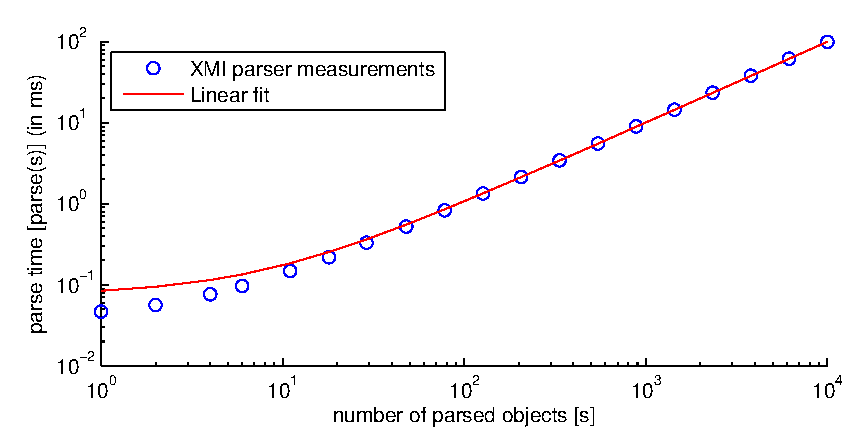
\includegraphics[width=\linewidth]{figures/emfParsePerf}
\caption{EMF's XMI parser performance.}
\label{fig:emfParsePerf}
\end{minipage}
\hspace{0.02\linewidth}
\begin{minipage}[b]{0.48\linewidth}
\centering
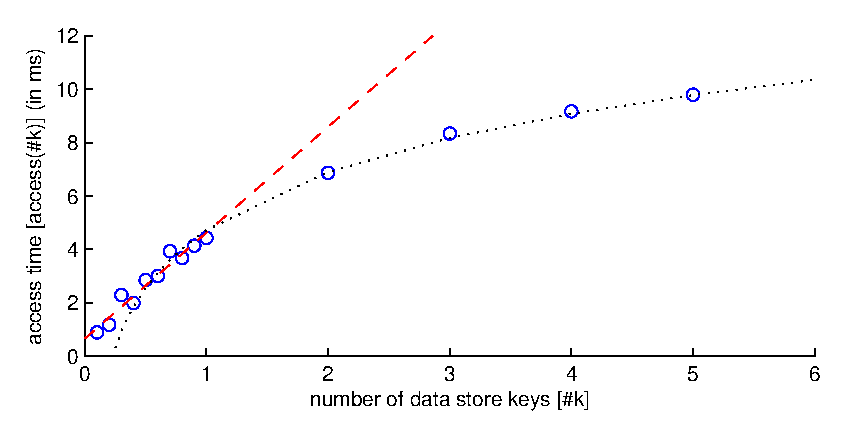
\includegraphics[width=\linewidth]{figures/hbaseAccessPerf}
\caption{HBase accesses performance.}
\label{fig:hbaseAccessPerf}
\end{minipage}
\end{figure}

 
Now, we can discuss the influence of fragment size $f$ on $t_{m,f}(l)$. First, we use a model of size $m=10^6$ and vary $f\in\{10^0,\dots,10^6\}$. Fig.~\ref{fig:theoryTimesSmall} shows the computed times $t$ over loaded model objects $l$ for the different fragment sizes $f$. We can observe four things. First, there is no optimal fragment size. Depending on the number of loaded objects, different fragment sizes are optimal. But intermediate fragment sizes provide good performance. With fragment size $f=10^2$ for example, all partial loads take three times the optimal time at most. Second, total fragmentation ($f=1$) requires roughly 100 times more time than optimal fragmentation, when larger numbers of objects $\ge 10^2$ are loaded. Thirdly, no fragmentation ($f=m$) is only a time efficient option, if we need to load almost all of the model. But in those cases no fragmentation is usually not practical for memory issues. Fourthly, for small partial models total fragmentation is far better than no fragmentation, for large partial models no fragmentation provides better performance.

\begin{figure}
\centering
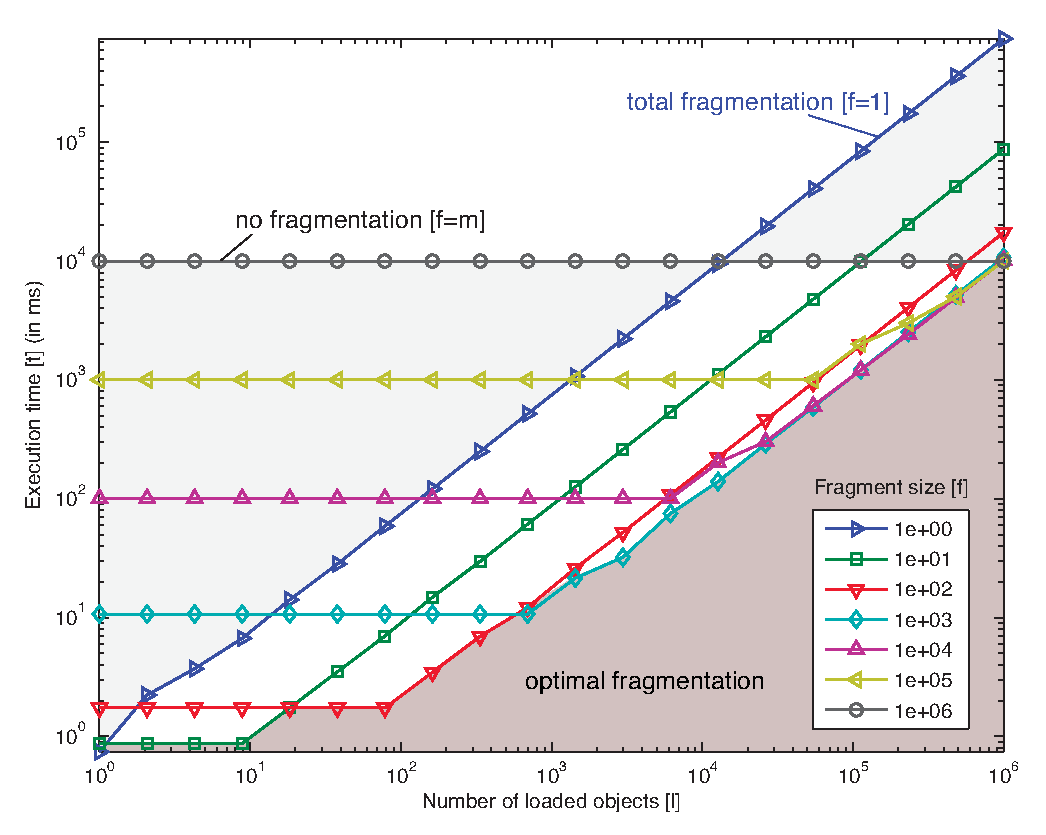
\includegraphics[width=0.65\linewidth]{figures/theoryTimesSmall}
\label{fig:theoryTimesSmall}
\caption{Computed execution times for partial loads from a model with $10^6$ objects and fragmentations of different granularity.}
\end{figure}

%Fig.~\ref{fig:theoryContour} shows the same data as contour plot. The largest partial models can be loading if the loaded parts have the same size as the fragments $l=f$. Fig.~\ref{fig:theoryTimesLarge} shows times for a larger model with $m=10^9$. Intermediate fragment sizes are still good fragment sizes. Such large models produce large number of database keys for total fragmentation, but the parsing overhead $parse(0)>0$ has obviously an larger influence than growing access times. Thus the plot for total fragmentation is still a line, and for large number of loaded objects, the plot for all fragment sizes are parallel.

%\begin{figure}[b]
%\begin{minipage}[b]{0.48\linewidth}
%\centering
%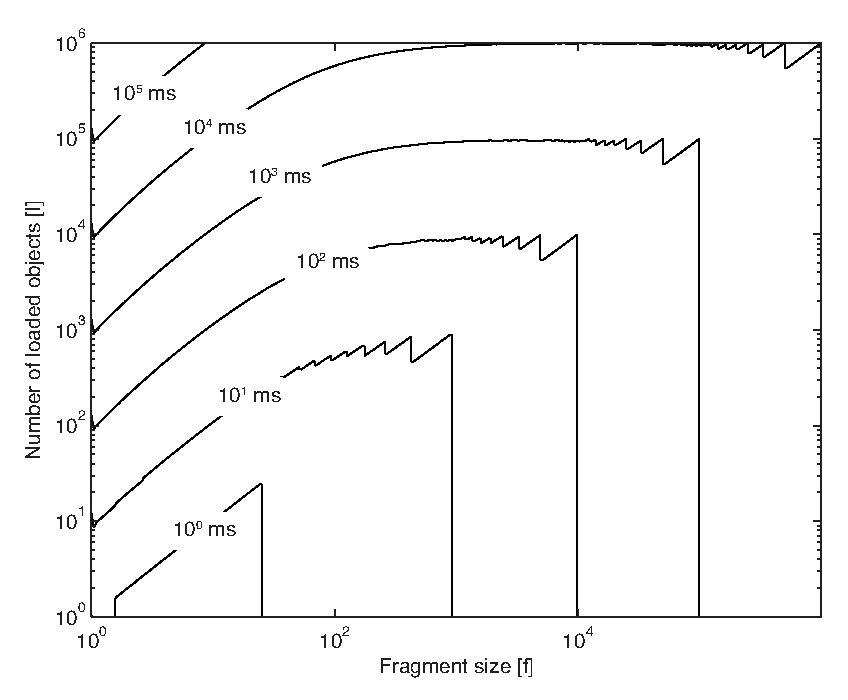
\includegraphics[width=\linewidth]{figures/theoryContour}
%\caption{Contour plot. Shows which $(f,l)$ have the same costs $t$.}
%\label{fig:theoryContour}
%\end{minipage}
%\hspace{0.02\linewidth}
%\begin{minipage}[b]{0.48\linewidth}
%\centering
%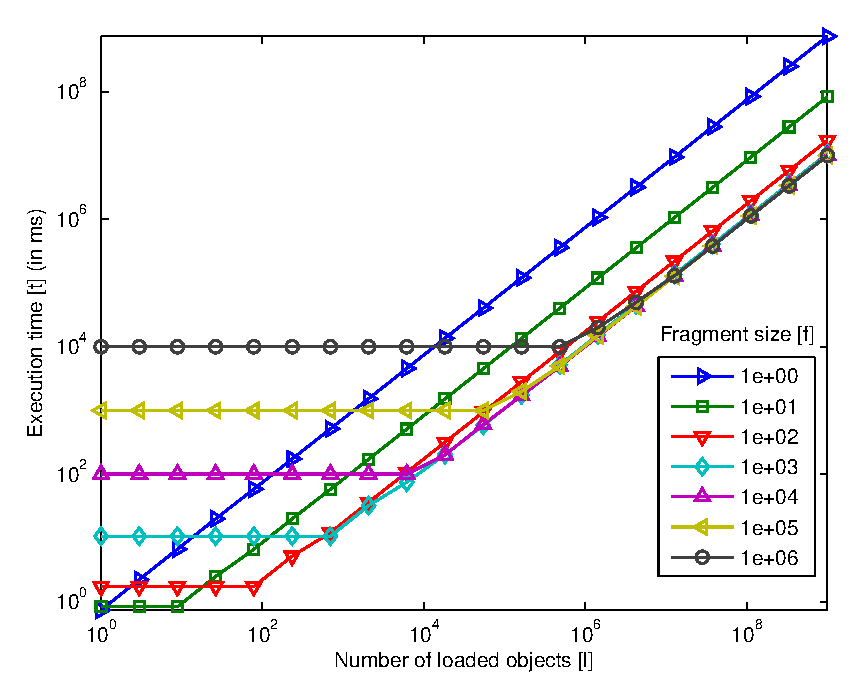
\includegraphics[width=\linewidth]{figures/theoryTimesLarge}
%\caption{Computed partial load times for a model of size $10^9$.}
%\label{fig:theoryTimesLarge}
%\end{minipage}
%\end{figure}
\section{Implementation of Model Fragmentation}
\label{sec:implemention}

In previous sections, we introduced model fragmentation, a specific fragmentation strategy, and the theoretical merits of fragmentation. In this section, we present a framework that realizes model fragmentation and implements the meta-model based fragmentation strategy. The framework is called \emph{EMFFrag}.

The rational behind EMFFrag is to (re)use EMF resource as much as possible. EMF resource already realize partial model persistence, they manage inter-resource references through proxies, they lazy-load, can be added and removed, objects can be moved between resources, etc. EMFFrag only uses and specialized the existing implementations of EMF resources.

\begin{figure}
  \centering
  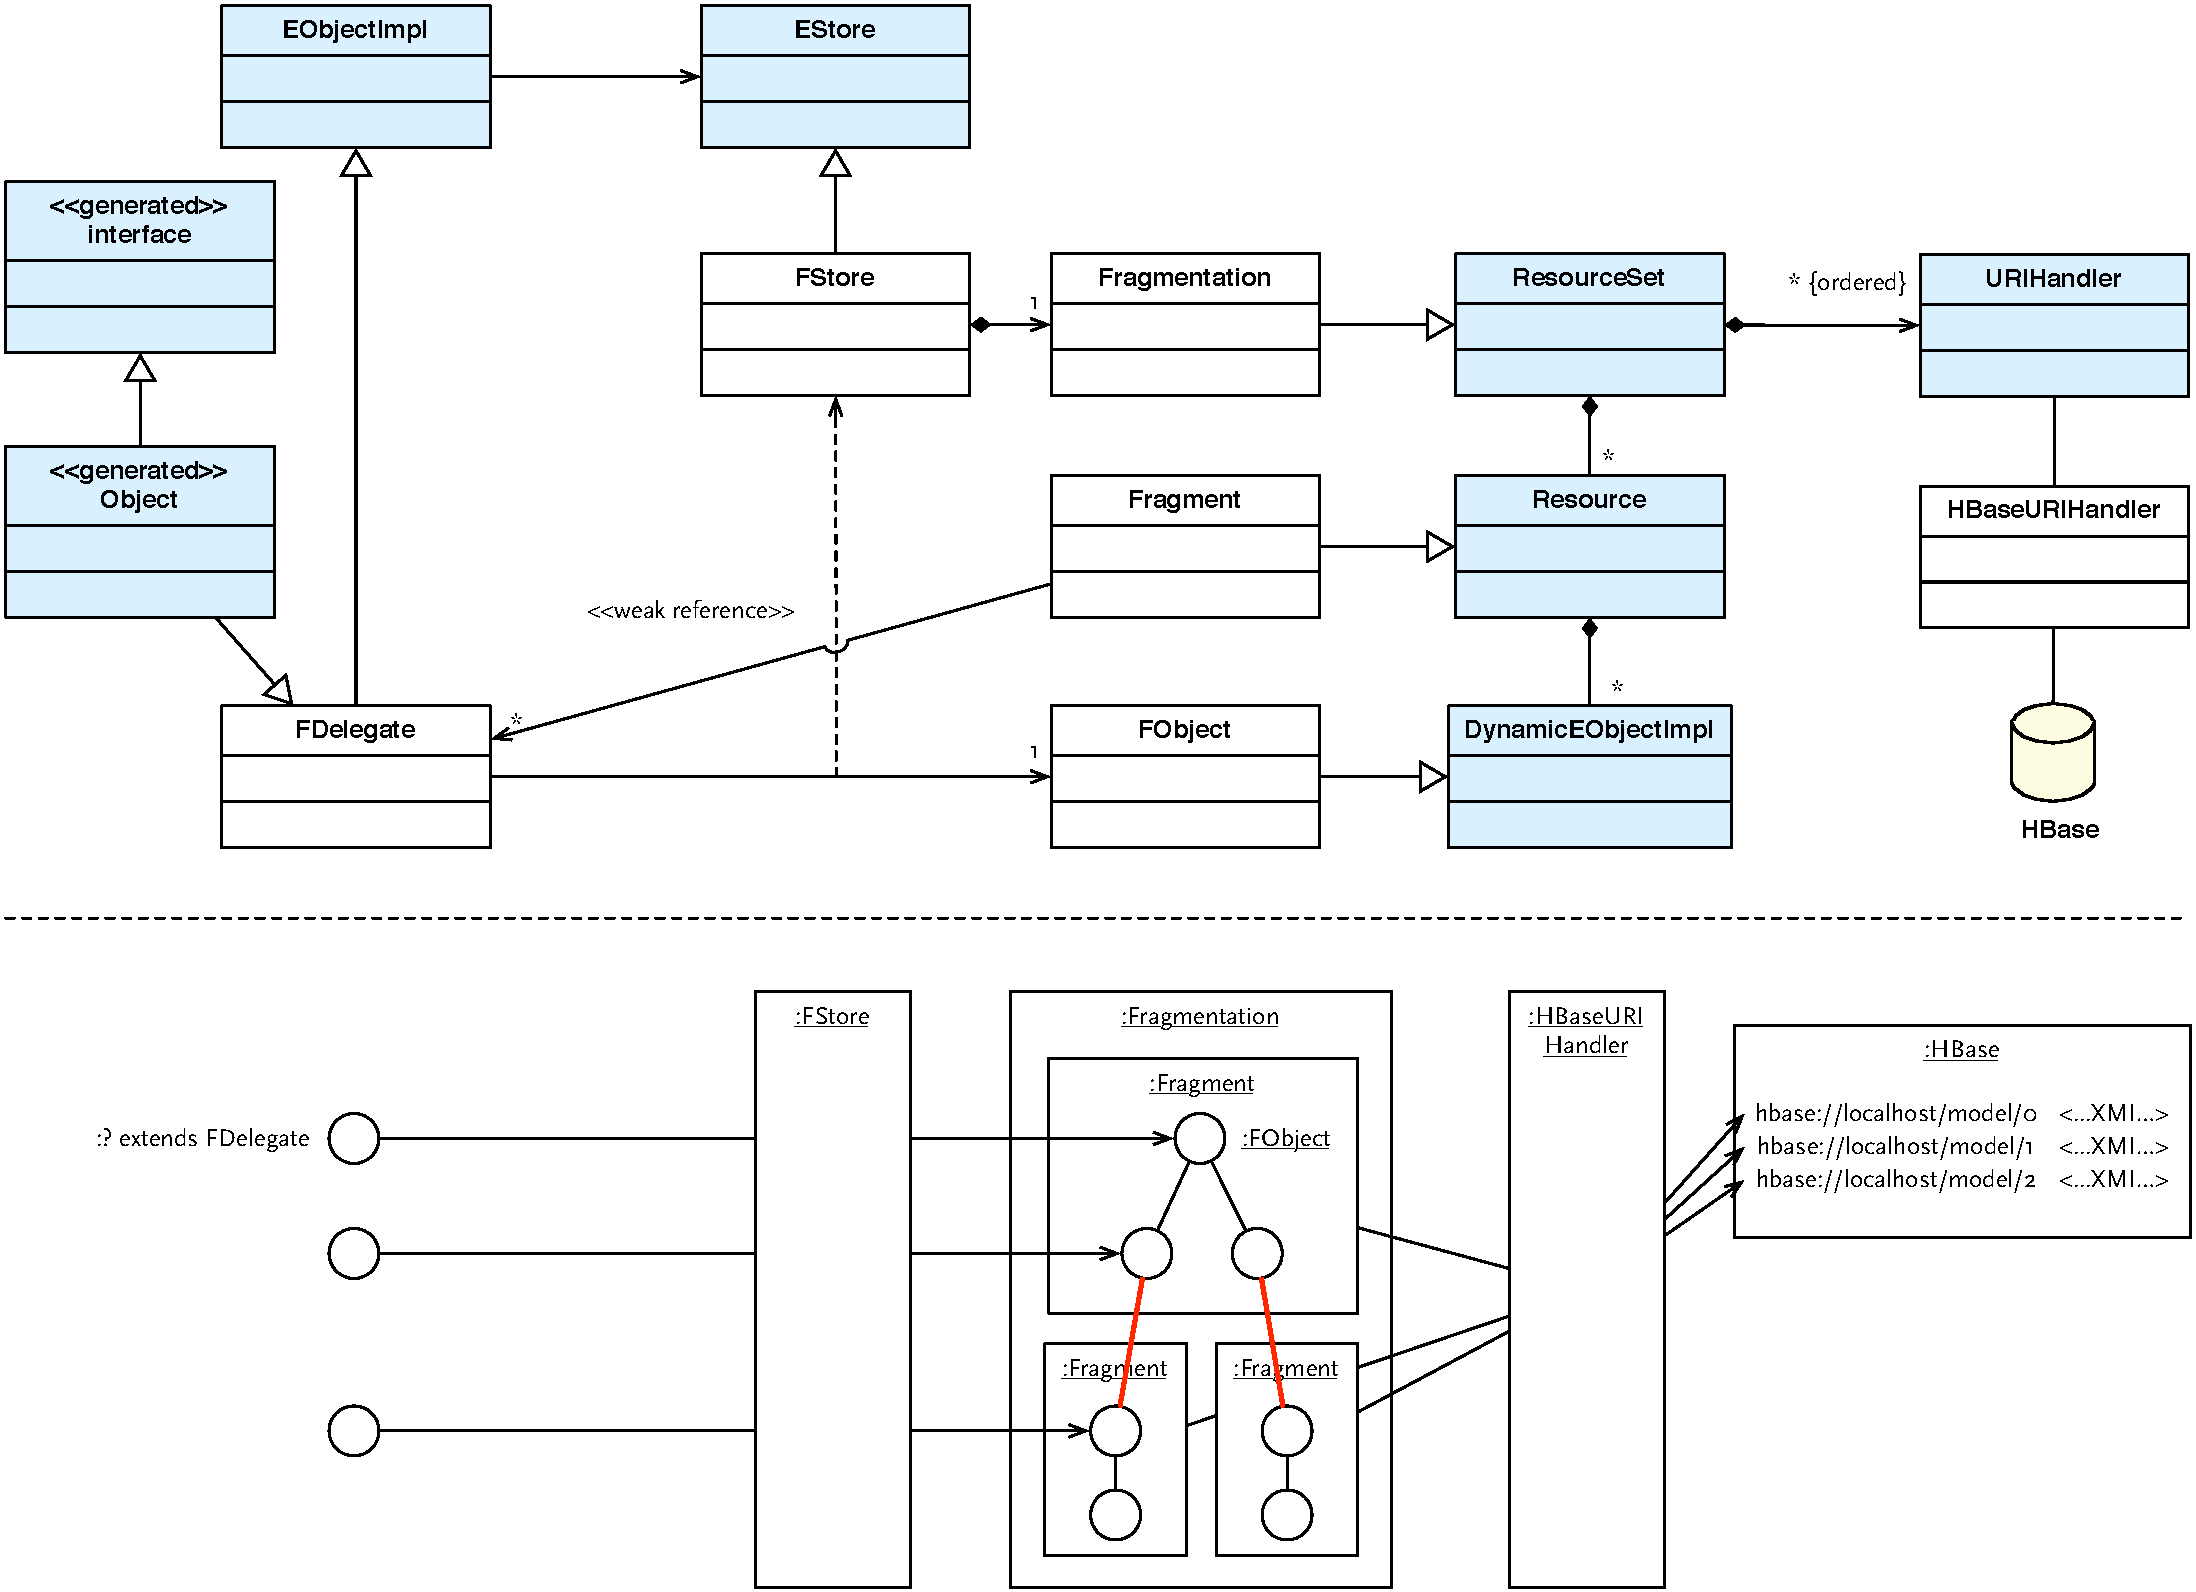
\includegraphics[width=\linewidth]{figures/architecture}
  \caption{EMFFrag architecture and example fragmentation.}
  \label{fig:architecture}
\end{figure}

Fig.~\ref{fig:architecture} illustrates EMFFrag's architecture and operation.

In EMFFrag a fragmentation is realized as a resource set, and fragments as resources. Different to EMF resources, fragmentations and fragments are completely hidden from the framework user (transparency). The fragmented model is internally realized though dynamic (meta-model independent) EMF objects. These internal objects are also hidden from users. Users access the model through generated (i.e. meta-model based interface) and stateless delegates. The delegates delegate all feature accesses to an EStore implementation, which delegates all calls to the corresponding internal object.  The store translates between delegates and internal objects: parameters are unwrapped from delegates to internal objects, and return values are wrapped from internal objects to delegates.

If a delegate was created by the user, the initial internal object is created, the first time the user gives the delegate to the store. Delegates are cached by fragments through Java weak references. If the store has to deliver an internal object to the user as delegate, the delegate is either cached in the fragment or created and cached.

This rather complex internal object and delegate architecture allows to recognize fragments that are no longer used. Once the weak reference cache of an fragment has lost all reference to cached delegated, it can be assumed that the user lost all references to all fragments. The fragment can be safely unloaded without destroying remaining delegates. 

The store recognizes when an object is added to (or removed from) a feature that is marked as inter-fragment reference feature in the meta-model. In this cases, EMFFrag creates a new fragment (or deletes a fragment) and moves the object into the new fragment. EMF's containment proxies handle everything else automatically. 

All fragments persist themselves through the regular URIConverter and URIHandler API. EMFFrag registers a specific URIHandler that maps fragment URIs to entries in an HBase key-value store. Fragments are lazy loaded through the regular EMF implementations. When a fragment is unloaded, it is saved (if changed). We extended the regular EMF unload behavior: EMFFrag does not only proxyfy all objects, but also removes all intra-fragment references. This allows the Java gargabe collecter to completely remove unloaded fragments.

Further fragment caching allows maintain unloaded caches on a LRU-basis for potential re-use. 

\section{Evaluation}
\label{sec:evaluation}

This section has two goals. First, we want to compare our fragmentation approach to other model persistence frameworks. Secondly, we want to verify our findings from section~\ref{sec:gains}. 
All measurements were performed on a Computer with Intel Core i5 2.4\.GHz CPU, 8 GB 1067 MHz DDR3 RAM, running Mac OS 10.7.3. All experiments were repeated at least 20 times, and all present results are respective averages. Code executing all measurements and all measured data can be downloaded as part of EMFFrag~\cite{EMFFragProject}.

\subsection{Fragmentation Compared to other Persistence Frameworks}

To compare fragmentation to EMF XMI, CDO, and Morsa, we measured execution time for the abstract modeling task. To analyse traverse and query, we used example models from the Grabats 2009 contest~\cite{grabats} as benchmarks. Those were already used to compare Morsa with EMF XMI and CDO here~\cite{morsa2011}. There are five example models labelled \emph{set0} to \emph{set4} and they all model Java software based on the same meta-model. Please note: even though the models increase in size, their growths is not linear. To measure the last task create/modify, we use simple test models, because importing Grabats' large XMI models files does not allow effective separation of loading the models with EMF and storing them with the respective persistence framework. We don't provide any comparative measures for partial loads. Partial load performance is indirectly covered by the measures on queries, which required to partially load the Grabats models. Furthermore, partial loads are extensively measured for EMFFrag in the next section.

Fig.~\ref{fig:grabatsFragments} shows the number of fragments that each framework produces for each model. Morsa and CDO implement total fragmentation and the number of fragments is also the number of objects in the model. For EMF XMI there is always only one fragment, because it implements no fragmentation. For EMFFrag, we provided two different meta-model based fragmentations. The first one puts each Java compilation unit and class file into a different fragment (EMFFrag coarse). The second one additionally puts the ASTs for each method block into a different fragment (EMFFrag fine). The number of fragments differs significantly for \emph{set2} and \emph{set3} which obviously contain a lot of method definitions. 

We could not measure CDO's performance for \emph{set3} and \emph{set4}: the models are to large for a single CDO transaction, and circular cross-references do not allow to import the model with different transactions.

\begin{figure}[ht]
\begin{minipage}[b]{0.48\linewidth}
\centering
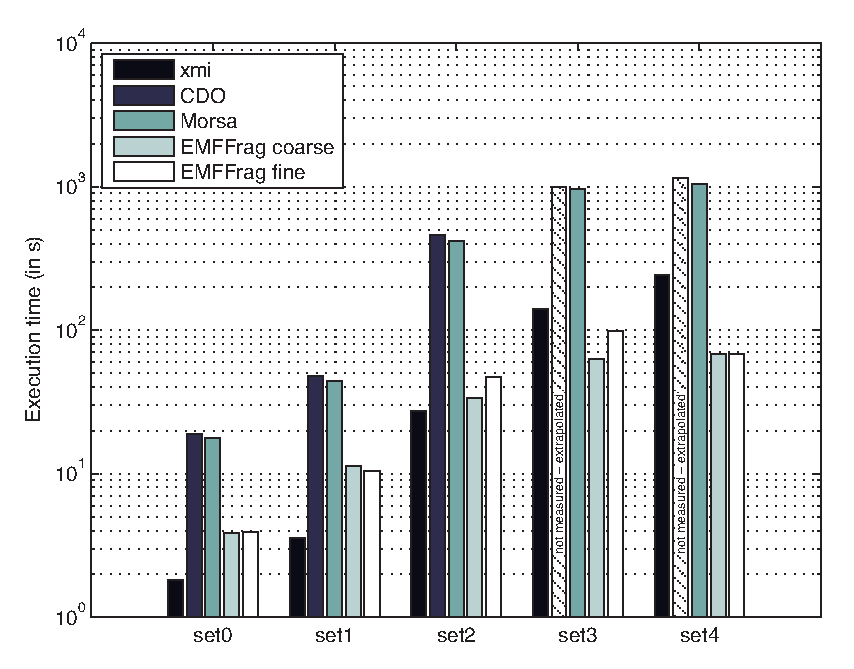
\includegraphics[width=\linewidth]{figures/grabatsTraverseTimeExtra}
\caption{Execution time for traversing the different Grabats models with the different persistence solutions.}
\label{fig:grabatsTraverseTime}
\end{minipage}
\hspace{0.02\linewidth}
\begin{minipage}[b]{0.48\linewidth}
\centering
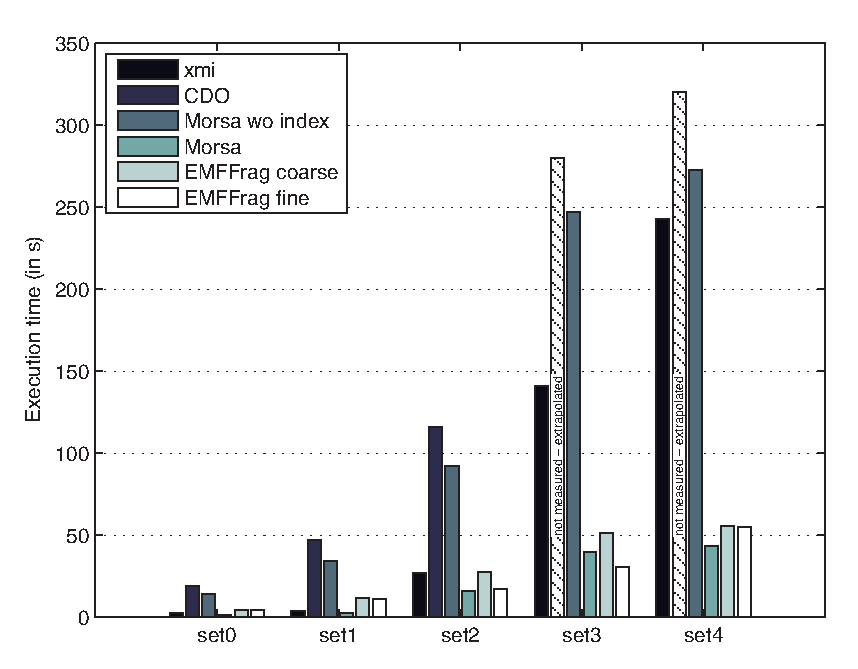
\includegraphics[width=\linewidth]{figures/grabatsQueryTimeExtra}
\caption{Execution time for querying the different Grabats models with the example query.}
\label{fig:grabatsQueryTime}
\end{minipage}
%\end{figure}
%\begin{figure}[ht]
\begin{minipage}[b]{0.48\linewidth}
\centering
\vspace{0.04\linewidth}
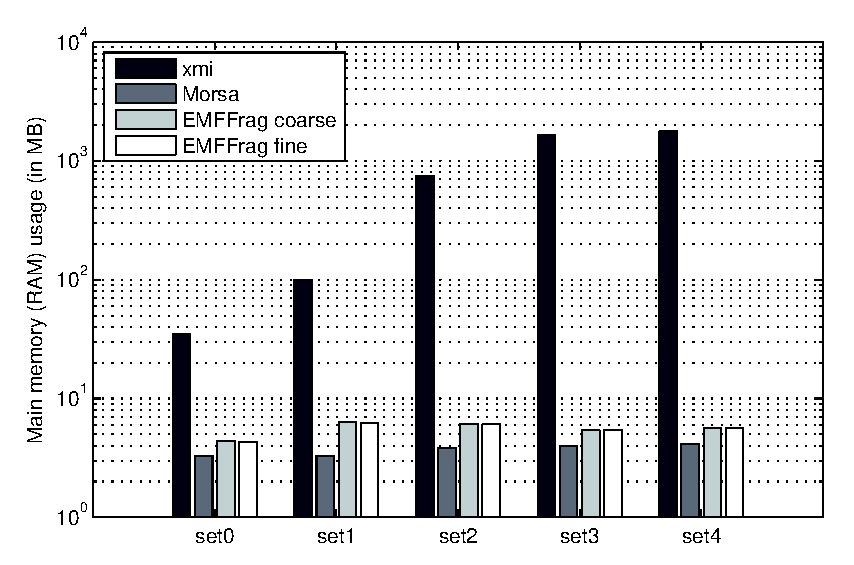
\includegraphics[width=\linewidth]{figures/grabatsTraverseMem}
\caption{Memory usage time for traversing the different Grabats.}
\label{fig:grabatsTraverseMem}
\end{minipage}
\hspace{0.02\linewidth}
\begin{minipage}[b]{0.48\linewidth}
\centering
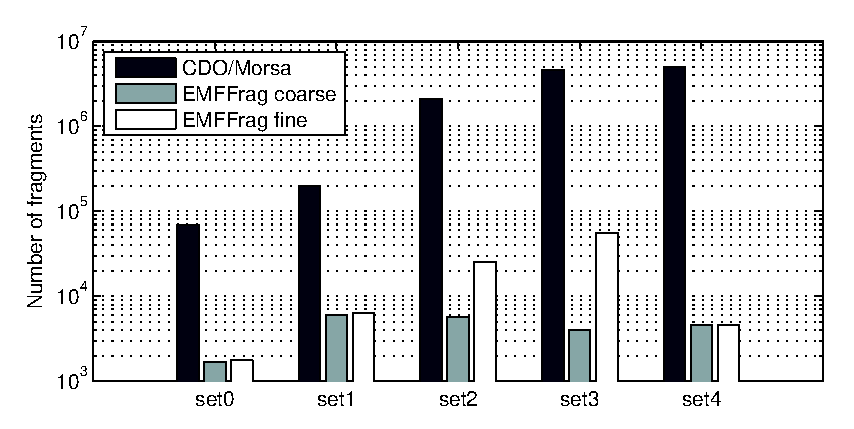
\includegraphics[width=\linewidth]{figures/grabatsFragments}
\caption{Number of fragments used by the different persistence solutions.}
\label{fig:grabatsFragments}
\end{minipage}
\end{figure}

\subsubsection*{Create/Modify} \markus{Big TODO: I need to measure this, describe the test models, plot results and testmeta-model and describe the results.}

\markus{Lorem ipsum dolor sit amet, consetetur sadipscing elitr, sed diam nonumy eirmod tempor invidunt ut labore et dolore magna aliquyam erat, sed diam voluptua. At vero eos et accusam et justo duo dolores et ea rebum. Stet clita kasd gubergren, no sea takimata sanctus est Lorem ipsum dolor sit amet. Lorem ipsum dolor sit amet, consetetur sadipscing elitr, sed diam nonumy eirmod tempor invidunt ut labore et dolore magna aliquyam erat, sed diam voluptua. At vero eos et accusam et justo duo dolores et ea rebum. Stet clita kasd gubergren, no sea takimata sanctus est Lorem ipsum dolor sit amet.}

\markus{Lorem ipsum dolor sit amet, consetetur sadipscing elitr, sed diam nonumy eirmod tempor invidunt ut labore et dolore magna aliquyam erat, sed diam voluptua. At vero eos et accusam et justo duo dolores et ea rebum. Stet clita kasd gubergren, no sea takimata sanctus est Lorem ipsum dolor sit amet. Lorem ipsum dolor sit amet, consetetur sadipscing elitr, sed diam nonumy eirmod tempor invidunt ut labore et dolore magna aliquyam erat, sed diam voluptua. At vero eos et accusam et justo duo dolores et ea rebum. Stet clita kasd gubergren, no sea takimata sanctus est Lorem ipsum dolor sit amet.}

\subsubsection*{Traverse} The execution times of CDO, Morsa, and EMFFrag are proportional to the size of the model (Fig.~\ref{fig:grabatsTraverseTime}). Times for EMF XMI grow faster than the model's sizes. Interestingly, Morsa and CDO both use total fragmentation and their respective execution times are very close. EMFFrag performs significantly faster: upto 10 times as fast as Morse and CDO. For models \emph{set2} and \emph{set3} (where the number of fragments differ largely between fine and coarse fragmentation) the fine fragmentation performs (not surprisingly) worse, since more fragments have to be loaded.

\subsubsection*{Query} The Grabats contest also provides an example query: find all Java type declarations that contain a static method which has this declared type as return type. Depending on the persistence framework, queries can be implemented in different ways. With EMF XMI and EMFFrag there are not indexes that would help to implement the query and we have to traverse the model until we found all type declarations. CDO allows to use SQL to query and Morsa provides a meta-model class to objects index. We measured both: executing the queries with these specific query mechanisms and with the previously mentioned traverse based implementation.

The results (Fig.~\ref{fig:grabatsQueryTime}: EMF XMI performs badly for large models. CDO and Morsa with SQL and meta-class index performs best. But even though EMFFrag needs to traverse the model its performance is similar to CDO and Morsa. For \emph{set3} and fine fragmentation, EMFFrag even outperforms Morsa's index. Remember, with the fine fragmentation, EMFFrag does not need to load any method bodies to execute the query (partial load). Using the traverse implementation, CDO's and Morsa's performance difference to EMFFrag is similar to the measures for model traverse (here we basically perform a partial traverse).  

\subsubsection*{Memory usage} During model traverse, we also measured the memory usage (Fig.~\ref{fig:grabatsTraverseMem}). EMF/XMI's memory usage is proportional to model size, because it needs to load the full models into memory. All other approaches need a comparable constant quantity of memory independent of model size.


\subsection{The Influence of Fragmentation on Partial Load Performance}

In section~\ref{sec:gains}, we looked at fragmentation analytically and provided a plot (Fig.~\ref{fig:theoryTimesSmall}) that describes the expected influence of fragmentation granularity on partial load execution times. Here, we create the same plot, but based on data measured with EMFFrag. For this purpose, we used a simple meta-model (ref. to Fig.~\ref{?}) and generated models of size $10^6$ with different fragment sizes $f$. We measured the execution times for loading parts of different sizes $l$. The results are presented in Fig.~\ref{fig:measureTimeExtra}.

\begin{figure}
  \centering
  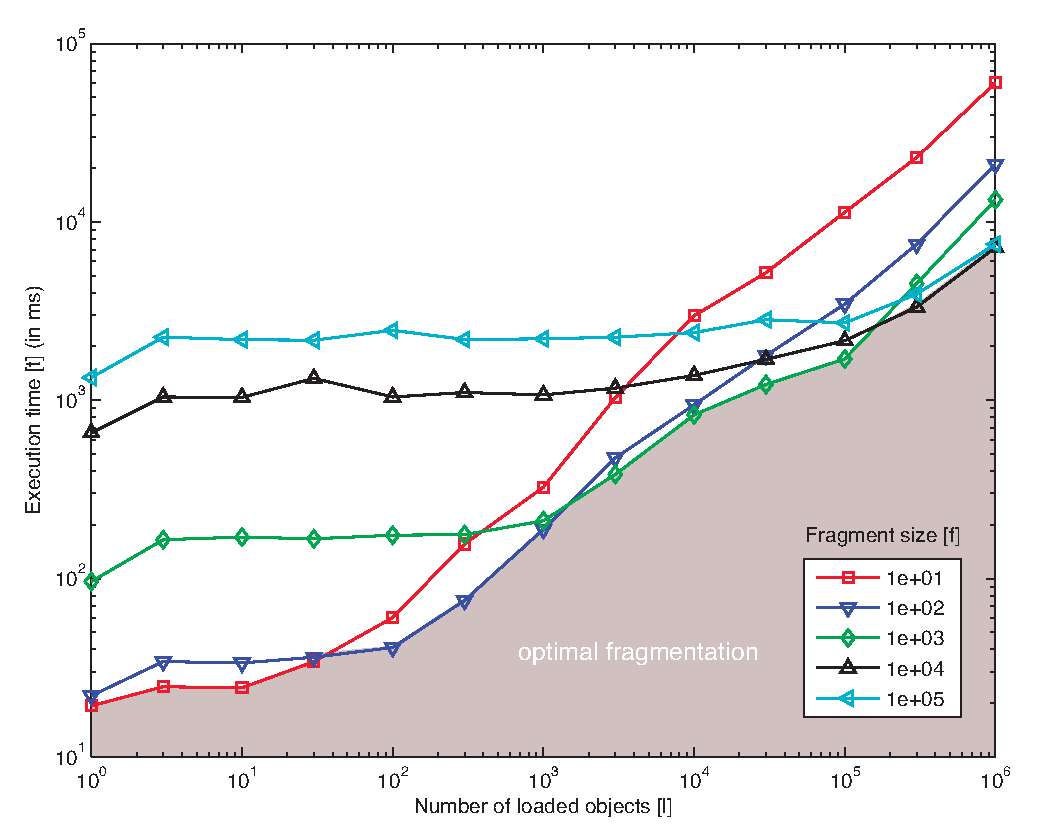
\includegraphics[width=0.65\linewidth]{figures/measureTimesExtra}
  \caption{Execution times for loading model parts with different fragmentation granularities.}
  \label{fig:measureTimeExtra}
\end{figure}

The plots show a similar picture with comparable values. Although, the measured times are generally larger probably due to additional EMFFrag implementation overhead that was not considered in our theoretical examination.
\section{Future Work} 
\label{future_work}

\subsubsection{Sorted and Distributed Key-Value Stores} 

Our fragmentation strategy is based on unsorted key-value store accesses with $\mathcal{O}log$ complexity. Neither our analysis, nor out  implementation EMFFrag, or our evaluation consider sorted key-value stores that allow to access sequential keys with constant time (scans). Neither did we consider distributed key-value stores which would allow parallel access. Key-value stores are easily distributed in peer two peer networks. This is done for two scalability reasons: replication (allows more users to access the same data in less time) and sharding (distributing data to allow faster and larger storage). Fragmentation can have an influence on both.

\subsubsection{Transactions}

If multiple user access/modify transactions become a necessity. Transaction can either be provided by the underlying data store (e.g. with Scalaris~\cite{ScalarisTransactions2008}) or can be implemented into EMFFrag. On non-distributed data stores, a common transaction pattern could be used. More interesting is explore the influence of fragmentation on transactions (and versioning), because the maximum granularity is determined by fragment size.

\subsubsection{Cross-References} 

EMFFrag persists containment references with URIs with a fragment ID pointing to the fragment that contains the reference objects. This does not work for cross references: when an object is moved, its URI changes and all referencing object use invalid URIs. For this reason EMFFrag needs to use a secondary index that maps object IDs to containing fragments. EMFFrag uses URIs with object IDs to persist cross references. To resolve such an URI, the secondary index is used to find the fragment that contains the object. Object IDs and secondary index are only maintained for objects that are actually cross references to keep the index small. 

In our analysis and evaluation, we did not examine the influence of cross references and corresponding indexes on performance. We have to expect that create/modify tasks are performed considerably slower, since two indexes have to be maintained. The impact on traverse, query, or partial loads, on the other hand, should be minimal.

\subsubsection{Large Value Sets}

In large models, single objects can become very large themselves if they hold large sets of attribute values and references. CDO maps an object's feature values to individual entries in a database table and can manage such objects, but does so slowly. EMFFrag (and Morsa), on the other hand, consider objects as atomic entities and large object become a performance burden too. We need to extend the fragmentation idea to large value sets. Similar to all consideration in this paper, these strategies for large value sets have to be optimized and evaluated for the abstract tasks manipulation, iteration (traverse), indexed access (query), and range queries (partial load). 

\section{Conclusions}\label{sec:conclusions}

Large software models consist of upto $10^9$ objects. Models from other application can have a size upto $10^{12}$ objects. Traversing models and loading larger aggregates of objects are common tasks (section~\ref{sec:applications}). Depending on fragment size, partially loading models can be done faster than loading whole models or loading models object by object. There is no optimal fragment size, but intermediate fragment sizes provide a good approximation  (sections~\ref{sec:gains} and~\ref{sec:evaluation}). We provide a persistence framework that allows automatic and transparent fragmentation, if appropriate containment features are marked as fragmentation points in the meta-model (sections~\ref{sec:fragmentation} and~\ref{sec:implemention}). We compared our framework to existing frameworks (EMF XMI, CDO and Morsa) and our framework performs significantly better for creating/manipulating, traversing, and partially loading models. Execution times are 5 to 10 times smaller. Model queries (that favour object-by-object based model persistence with indexes, such as in CDO and Morsa) can be executed with comparable execution times (section~\ref{sec:evaluation}). Model fragmentation also determines the granularity of transactions, which can be a disadvantage. Further problems are single objects with features that can hold large value sets; the fragmentation approach has to be extended for fragmentation of such value sets (section~\ref{sec:future_work}). Our framework stores fragments in key-value stores. Those scale easily (both replication and sharding is supported) and integrate well in peer-to-peer computation scheme (e.g. map-reduce). Fragmentation therefore prepares very large models for modelling in the cloud applications (section~\ref{sec:related_work}).

\clearpage
\bibliography{bibliography}

\end{document}
